\section{Computer Plot}

Using a computer to plot the graph of a function is easy. You can use
software such as MATLAB to easily plot graphs, inspect them and create
vector or raster images of them.

I have used GNU Octave because of avaliability, however the scipt is 
MATLAB compatible.

\lstinputlisting[language=Octave]{computer/matplot.m}

\begin{center}
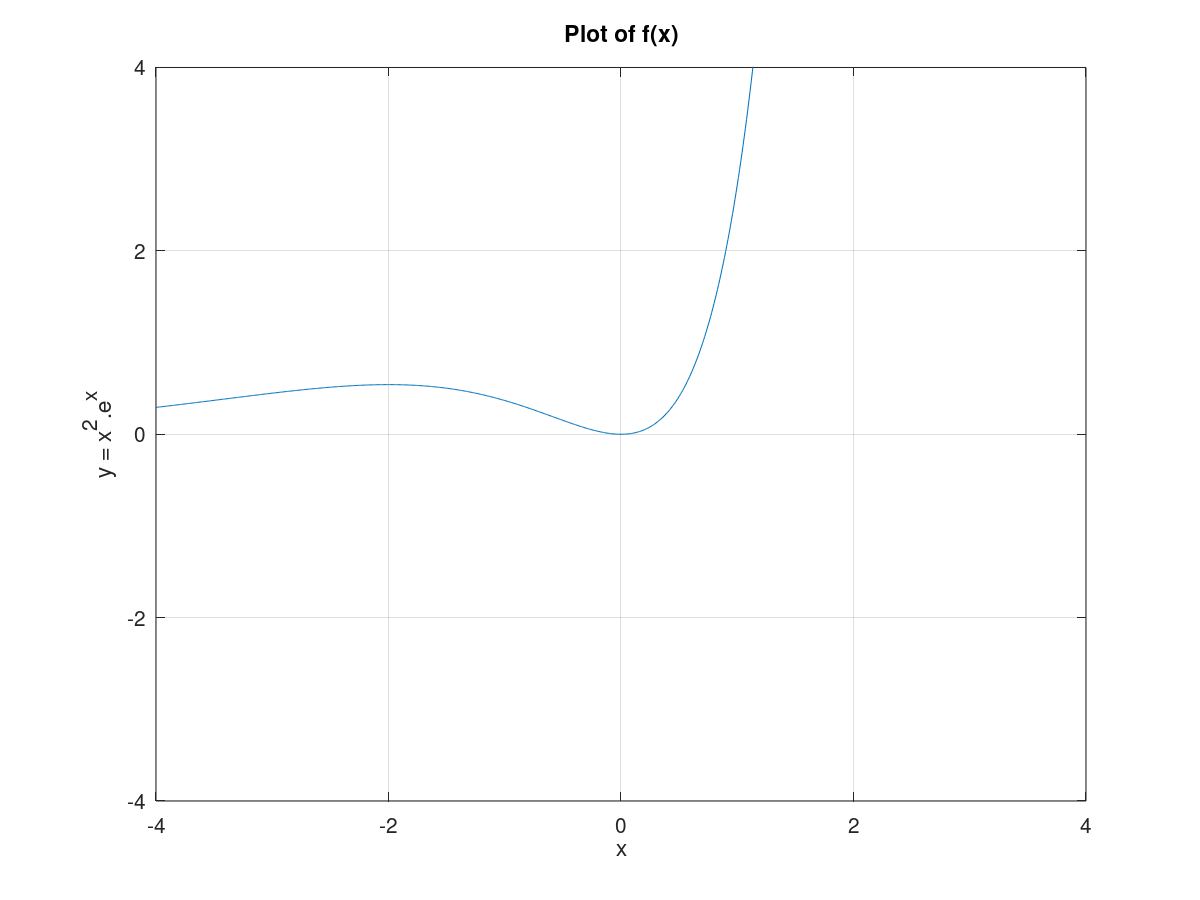
\includegraphics[width=118.8mm]{computer/plot.png}
\end{center}

For the comparison of the plots, the figures are simply 
overlayed in graphics editing software.

\begin{figure}[h!]
    \centering
    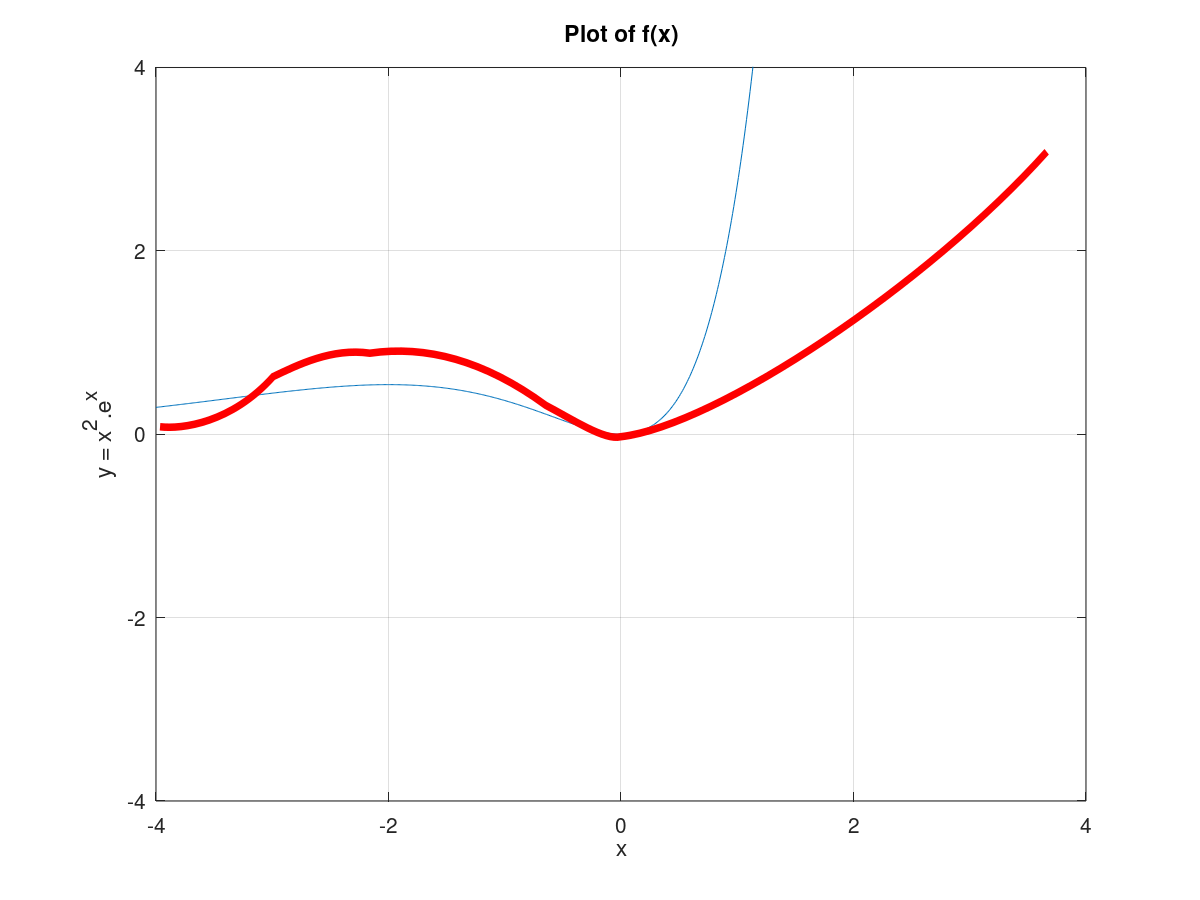
\includegraphics[width=118.8mm]{computer/comparison.png}
    \caption{The figures overlayed in software.}
    \label{compare}
\end{figure}

Despite the inaccuracies of the hand plot, Figure \ref{compare} clearly
shows we were able to plot the function successfully.In hand plots,
features of the function are exaggerated unless done in another
approach. Due to this fact, hand plots should not be used in geometric
proofs, but as a reference.

However our hand plot is not missing any feature of the graph. All the 
inflection points, local minimums, local maximums, and intersections are
visible.